\chapter[SCP-150 忒修斯之船]{
SCP-150 Ship of Theseus\\
SCP-150 忒修斯之船
}

\label{chap:SCP-150}

\bb{项目编号:}SCP-150

\bb{项目等级:}Keter

\begin{figure}[H]
\centering
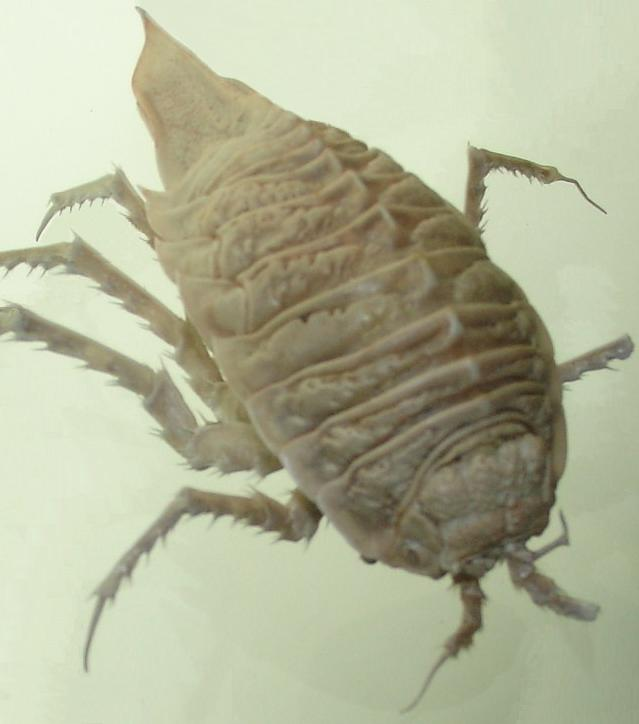
\includegraphics[width=0.5\linewidth]{images/SCP-150.jpg}
\caption*{从D13732脑内取出的SCP-150样本,放大20倍}
\end{figure}

\bb{特殊收容措施:}用于研究的SCP-150感染者应当被保存在Ⅲ级生化危害收容单元中,每个单元不超过一个实体。SCP-150的样本应被收容在site-42的传染性材料实验室中,置于真空封存的细颈瓶内。标准的病原体处理进程应随时被遵照。任何在收容以外发现的SCP-150样本将被焚化。

\bb{描述:}SCP-150是一种专性寄生虫,外观类似食舌虱(Cymothoa exigua,即缩头鱼虱)。但适应在其部分的生命进程中与人类形成共生关系。一旦与一个人类接触,SCP-150将会将自身深深的埋入寄主的血肉中。经过大约七天之后,它将会挖洞钻入宿主的体内,并导致一系列生理改变。

最显著的变化是距感染部位最近的肢体逐渐变为几丁质的附肢。当SCP-150消耗寄主的血肉时, 他将分泌出物质用以代替并增大寄主肢体且不造成排异反应。怀疑SCP-150能够分泌麻醉物质和免疫抑制素以抑制人体对变化的反应。此外,SCP-150分泌出的神经组织能够与宿主的神经系统结合。在这个过程结束之前,寄主将能不受阻碍地控制被感染的肢体,甚至在强壮、灵活程度以及恢复能力上有所提高。

在一到两周之后,SCP-150会增殖,从被同化的血管中吸收营养物质并在其中产卵\footnote{假定SCP-150能够营自养生活。}。卵将随血液的流动在人体内移动直到大部分卵死去,剩余足够存活的卵将开始在宿主身体的其他部位增殖并将其加以改变。尽管这一过程中被感染者报告了不适和偶然的运动控制缺失,他们常常不会意识到所述不适的诱因。为何SCP-150的后代不会为了空间和资源相互竞争以及它们的同化过程怎样不引发机体细胞的信号机制和过程依旧成谜。在这个同化过程中SCP-150不断增殖:当肺部被同化后,更多的卵产生并通过感染者的咳嗽传播。尽管一次能产生多达10000个卵,预计只有1\%的个体能够进入另一个宿主的体内,而已经进入宿主体内的个体也只有1\%能够从宿主的免疫应答中存活。

尽管SCP-150必然导致同化作用和中央神经系统(包括脊索和大脑)的转变,宿主的意识和举止似乎不受影响。因为受感染者意识不到SCP-150的存在,他们往往声称感受不到在特定感觉和能力方面的改变与提高,所以与SCP-150感染者的交流几乎没有收集到信息。当受感染者意识到此种感染是其机体改变的原因时,他们并没有表现出消极情绪且常常对此表现出积极性。

\bb{附录150-E:}两位D级人员,D-13732和D-016002,被SCP-150感染并被允许经历感染的全部过程。为了检验感染的全部影响,探索性的神经外科检查在两者身上被实施。D-13732被安乐死:他的神经组织完全被更小的SCP-150个体取代。组成其脑部物质的个体被取出保存并用于D-016002的实验。

以下的颅内减压术和脑白质切除手术由Harlan Sun博士、Wendy Robin博士、Alex Harlow博士对D-016002进行。完整副本如下:

\begin{scpbox}

\bb{<开始记录,21:43>}

\ii{D-016002被部分麻醉以使其在最初对头骨的钻孔中保持麻木。过程十分平静,尽管Harlan博士报告在颅骨上的钻孔和割出切口的过程中受到了比他预计更少的阻力。在移除骨片、使脑膜暴露的的过程中,大量SCP-150的更小实体被观察到位于原本是大脑所在位置的颅腔中。Harlow向Robin报告这一现象,后者指示前者开始采访过程,与此同时后者按照图像投影标出D-016002的脑部区域。}

\bb{Dr. Sun:}你的名字?

\bb{D-016002:}mako {[}数据删除]。

\bb{Dr. Sun:}说个能坐的东西?

\bb{D-016002:}椅子(chair)。

\bb{Dr. Sun:}草是什么颜色?

\bb{D-016002:}绿色。

\bb{Dr. Sun:}一加一等于几?

\bb{D-016002:}二。

\bb{Dr. Robin:}我们已经标出了韦尼克区\footnote{控制语言理解和使用的脑部区域。}的大致位置。

\bb{Dr. Harlow:}谢谢,Sun博士。我将从这个区域取出一些样本。

\ii{Harlow博士小心的从脑膜上开出一个切口并用镊子从中取出了一些样本。他将每个个体放进一个玻璃小瓶中并用塞子塞住,将其放在一个邻近的置物台上。每个个体只有在被移动时才表现出应激反应和蠕动。这个过程大约持续了10分钟,在这期间Sun博士重复询问D-016002同样的问题。当Harlow博士取出了大概100个个体后,他示意Sun继续。}

\bb{Dr. Sun:}说个能坐的东西。

\bb{D-016002:}呃,呃,座椅(seat)。

\bb{Dr. Sun:}草是什么颜色?

\bb{D-016002:}绿色?

\bb{Dr. Sun:}一加一等于几?

\bb{D-016002:}…二。

\bb{Dr. Sun:}记录D-016002的回应稍微变慢了。这表明她颅腔内的个体事实上表现为神经元类似物,尽管每个个体等价于多少个神经元尚不清楚。

\bb{Dr. Harlow:}我将把从D-13732处取得的一个神经系统样品放入D-016002体内。从D-13732体内取得的个体用发光性放射涂料标记来使其能在之后被区分出来。

\bb{Dr. Sun:}说个能坐的东西。

\bb{D-016002:}沙发。

\bb{Dr. Sun:}草是什么颜色?

\bb{D-016002:}蓝色。

\bb{Dr. Sun:}一加一等于几?

\bb{D-016002:}二。

\bb{Dr. Sun:}十乘十一等于多少?

\bb{D-016002:}一百一十一。

\bb{Dr. Sun:}D-016002的回应回到了正常速度。这表明可能在宿主个体间自由地交换150个神经组织能不受阻碍。我们将开始最后一步,D-016002,你将会被全身麻醉。

\ii{(D-016002被施以全麻,这耗时几秒以开始。)}

\bb{Dr. Sun:}感染者现在处于全麻状态下。Harlow博士,你可以开始组织的取出了。最后一步中,我们将打算把D-016002的脑组织完全换成D-13732的。之前在D-13732的颅腔探索中,我和Harlow博士观察到连接她大脑和脊髓的个体没有受到任何方式的保护,并且事实上这些实体似乎在与脑内的其他实体不断进行换位。我们将看看这种兼容性能扩张多远。

\ii{(接下来的一个小时一片寂静,三位博士移去了D-016002的颅骨顶部并开始将她的脑部移入一个大的玻璃容器中。)}

\bb{Dr. Sun:}移取完成。D-016002的大脑被成功移出。Harlow博士现在将把D-13732的大脑移入D-016002的开放颅腔中。

\ii{(几分钟的沉寂。)}

\bb{Dr. Robin:}心率稳定。有脉搏和呼吸。再给它们一分钟……好了,我要唤醒她了。

\ii{(一阵暂停,Robin博士减少了麻醉剂量,D-016002醒了)}

\bb{Dr. Sun:}你的名字?

\bb{D-016002:}Michael {[}数据删除]\footnote{D-13732的名字。}。

\bb{Dr. Harlow:}(在背景音中能被轻微的听到)天哪。

\bb{Dr. Sun:}说个能坐的东西。

\bb{D-016002:}豆子袋。

\bb{Dr. Sun:}草是什么颜色?

\bb{D-016002:}绿色。

\bb{Dr. Sun:}一加一等于几?

\ii{(安静的环境下,麦克风侦测到一些晃动声。)}

\bb{Dr. Robin:}嘿!呃,Sun——

\bb{D-016002:}二。

\bb{Dr. Robin:}Sun,看!

\ii{(D-016002的大脑表现出自行移动,微微地前后移动。)}

\bb{Dr. Harlow:}哦?新东西……

\bb{Dr. Sun:}你感到身上有地方痛吗?

\bb{D-016002:}我胸口有点重。除此以外一切正常。

\bb{Dr. Sun:}听着不错。现在,十乘以——

\bb{D-016002:}嘿,我即使在手术前也常常感到精力充沛。但我现在有点累了。最近我开始在睡觉前锻炼了,但因为在这,我没法这么做。我能就休息一小会吗?

\bb{Dr. Sun:}休息?

\bb{D-016002:}就大概三五分钟。如果可以的话在这就行(D-016002的头顶部的一小部分发出了一阵咕咕声然后裂开了,在这部分合上之后,D-016002的大脑的几个部分自行缩了回去。D-016002的眼睛合上了。)

\bb{Dr. Sun:}那看上去不怎么样。(Robin博士从手术室离开了,离开时发出一阵干呕声。)

\bb{Dr. Harlow:}D-016——啊,D-13732 ,你还好吗?

\bb{D-016002:}啊?(哈欠)我很好,你问啥?

\end{scpbox}
